\chapter{Introduction}
\addcontentsline{toc}{chapter}{Introduction}
Today's processors have multiple cores and it's single core performance is improving only very slow because of physical limitations. On the other hand number of cores is still increasing and we can assume that it will continue. That's why developing parallel software is crucial for improving overall performance.

Parallelization can be achieved manually or using some framework designed for it. For example there are frameworks like OpenMP or Intel TBB. Department of Software Engineering at Charles University in Prague developed it's own parallelization framework called Bobox\cite{bobox}.

Bobox is designed for parallel processing large amounts of data. It was specifically created to simplify and speed up parallel programming of certain class of problems - data computations based on non-linear pipeline. It was successfully used in implementation of XQuery and TriQuery engines.

Bobox consists from runtime environment and operators. These operators are called boxes and they are C++ implementation of data processing algorithms. Boxes use messages called envelopes to send processed data to each other. 

Bobox takes as input execution plan written in special language Bobolang\cite{bobolang}. It allows to define used boxes and simply connect then into directed acyclic graph. Bobolang specifies the structure of whole application. It can create highly optimized evaluation, which is capable of using the most of the hardware resources.

Most used databases are relational databases. They are based on the view of data organized in tables called relations. SQL\cite{database} ("Structured query language") is very important language based on relational databases. It is used for querying data, modifying content of tables and also the structure of tables.

Architecture of planned SQL compiler is displayed in figure~\ref{fig:sqlarchitecture}. 
\begin{figure}[h!]
  \centering

    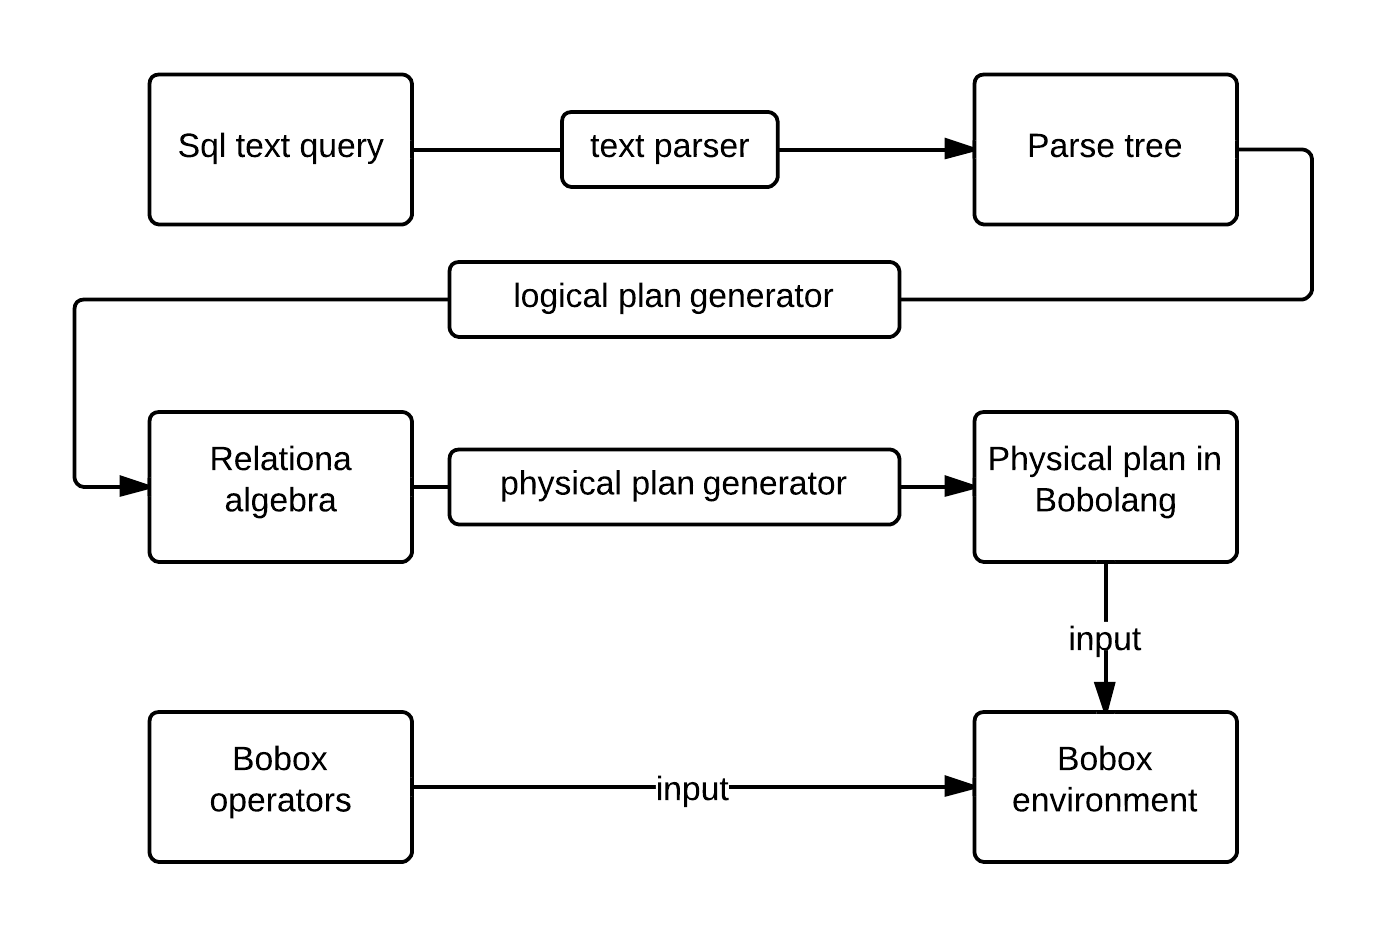
\includegraphics[width=1\textwidth]{sqlarchitecture}
    
      \caption{SQL compiler architecture.}
        \label{fig:sqlarchitecture}
\end{figure}
SQL query is written in text. This text is parsed into parse tree, which is transformed into logical query plan (Relational algebra). Relational algebra is then optimized and this form is used for generating physical query plan. Physical plan written in Bobolang is input for Bobox for execution. Physical plan is not enough, we need to also provide implementation of physical algorithms (Bobox operators).

Since SQL is a pretty complicated language, this thesis aim is only implementing optimization and transformation of logical plan into physical plan. This part is displayed as physical plan generator in figure~\ref{fig:sqlarchitecture}.


The main goal of this thesis is to implement part of SQL compiler. The input is query written in XML format in from of relational algebra. Program reads input and build relational algebra tree, which is then checked for semantic errors. Then we improve logical plan by pushing selection down the tree. From improved relational algebra tree we generate physical plan. In this phase we assign physical algorithm for every logical plan operator and we also choose order of joins. The output is execution plan for Bobox written in Bobolang.
